%  !TeX  root  =  user_guide.tex

% when the revision of a section has been finalized, 
% comment out the following line:
% \updatedisclaimer

\section{Plugin eVis}\label{sec:evis}

Il plugin eVis è stato sviluppato dalla 'Biodiversity Informatics Facility' del 'American Museum 
of Natural History's (AMNH) Center for Biodiversity and Conservation (CBC)' \footnote{Questa sezione 
è derivata da Horning, N., K. Koy, P. Ersts. 2009. eVis (v1.1.0) User's Guide. American Museum of
Natural History, Center for Biodiversity and Conservation. 
Disponibile all pagina web \url{http://biodiversityinformatics.amnh.org/}, rilasciato con licenza GNU FDL.} 

Nella nuova versione di QGIS, eVis è installato automaticamente; come tutti gli altri plugin può 
essere abilitato/disabilitato tramite il gestore dei plugin (Sezione \ref{sec:managing_plugins}).

Il plugin consta di tre moduli, Connessione Database, ID evento, Browser evento che permettono di collegare 
a vettori in QGIS foto ed altri documenti geocodificati (es. con coordinate X,Y o lat/long).  

\subsection{Browser evento}\label{evis_browser}

Il modulo mette a disposizione le funzionalità per visualizzare foto geocodificate collegate ad elementi
vettoriali della vista mappa di QGIS, come un layer di punti creati direttamente in QGIS o il risultato
di una query. Gli elementi vettoriali devono avere associati attributi che ne descrivono la localizzazione
ed il nome del file contenente le foto: opzionalmente l'orientamento della macchina fotografica. Il 
layer vettoriale deve essere caricato in QGIS prima di poter usare il Browser evento.

\minisec{Aprire il modulo Browser evento}\label{evis_launch_browser}

Per aprire la finestra di dialogo del modulo, cliccare su \toolbtntwo{event_browser}{Sfoglia eVis} oppure 
\mainmenuopt{Plugins} \arrow \dropmenuopt{eVis} \arrow \dropmenuopt{Sfoglia evento eVis}. 

La scheda \tab{Visualizza} serve a visualizzare le foto ed i relativi attributi. La scheda \tab{Opzioni}
contiene una serie di impostazioni del plugin. La scheda \tab{Configura applicazioni esterne} serve a
gestire una tabella di estensioni di file ed applicazioni associate per permettere ad eVis di visualizzare 
documenti ed altre immagini.      

\minisec{Scheda Visualizza}\label{evis_display_window}

La scheda \tab{Visualizza} è usata per visualizzare le foto ed i relativi attributi. 

\begin{figure}[ht]
   \centering
   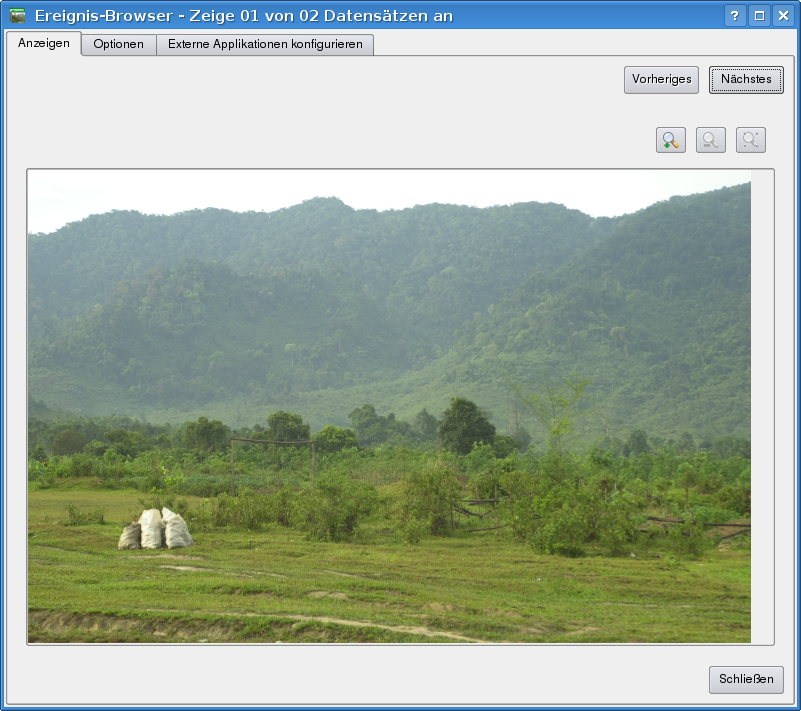
\includegraphics[clip=true, width=12cm]{evisdisplay}
   \caption{Scheda Visualizza di \emph{eVis} \nixcaption}\label{evisdisplay}
\end{figure}

\begin{itemize}[label=--]
\item \textbf{Area di visualizzazione dell'immagine}: è il riquadro inferiore della scheda.
\item \textbf{Ingrandisci}: ingrandisce l'immagine per avere più dettagli. Se l'immagine è troppo 
grande per l'area di visualizzazione, compaiono delle barre di scorrimento.
\item \textbf{Rimpicciolisci}: rimpicciolisce l'immagine.
\item \textbf{Zoom all'estensione massima}: visualizza l'immagine nella sua totalità.
\item \textbf{Finestra degli attributi}: è il riquadro superiore della finestra. Qui sono mostrate 
le informazioni del punto associato alla foto che si sta visualizzando. Se il file associato al punto 
non è un'immagine ed il tipo di file è definito nella scheda delle applicazioni esterne, facendo 
doppio-click sul suo percorso viene avviata l'applicazione adatta a gestire quel tipo di file.  
\item \textbf{Pulsanti per la navigazione}: usare i pulsanti \button{Precedente} \button{Avanti} per 
passare da un elemento all'altro.
\item \textbf{Indicatore elemento}: l'intestazione indica quale elemento è visualizzato ed il numero di
elementi disponibili.
\end{itemize}

\minisec{Scheda Opzioni}\label{evis_options_window}

\begin{figure}[ht]
   \centering
   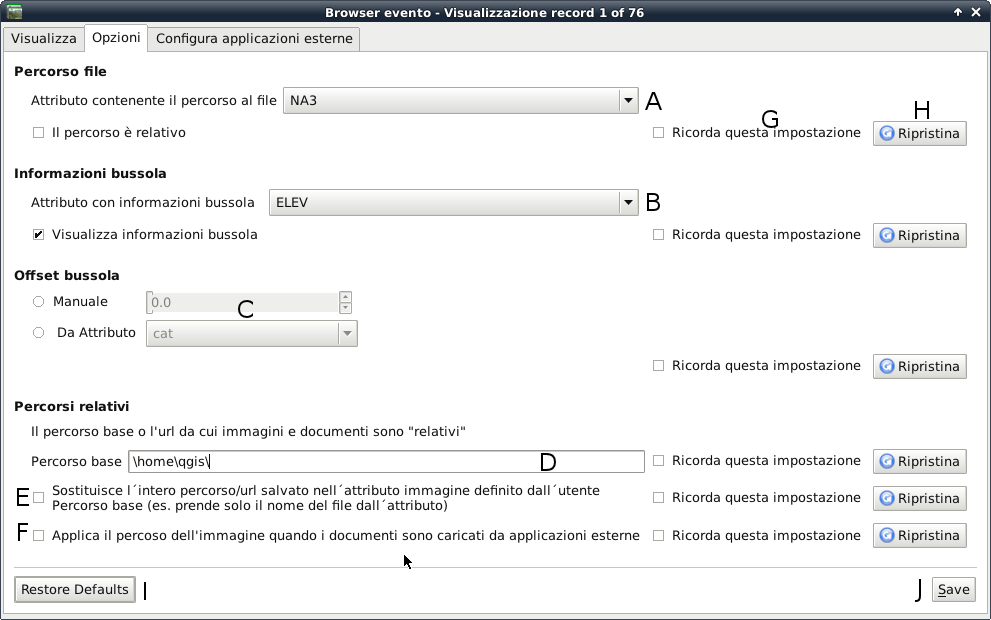
\includegraphics[clip=true, width=12cm]{evisoptions}
   \caption{Scheda Opzioni di \emph{eVis} \nixcaption}\label{evisoptions}
\end{figure}

\begin{itemize}[label=--]
\item \textbf{(A) Percorso file}: menu a tendina che permette di selezionare l'attributo contenente il 
percorso o l'URL della foto o altro documento da visualizzare. 
In caso di percorso relativo, attivare la casella di controllo \checkbox{Il percorso è relativo}: 
il percorso di base del percorso relativo può essere indicato nella casella di testo 'Percorso base'.
Informazioni di dettaglio sulle diverse opzioni per specificare la localizzazione di un file sono
disponibili nella Sezione \ref{evis_specifying}.
\item \textbf{(B) Informazioni bussola}: menu a tendina che permette di selezionare l'attributo contenente
l'orientamento della macchina fotografica.
\item \textbf{(C) Offset bussola}: può essere usato per compensare la declinazione. Attivare \radiobuttonon{Manuale}
per inserire i valori di offset della casella di testo oppure attivare \radiobuttonon{Da Attributo} per 
selezionare l'attributo contenente i valori di offset. La declinazione est deve essere inserita usando valori 
positivi: in valori negativi, invece, la declinazione ovest.
\item \textbf{(D) Percorso base}: il percorso di base utilizzato dal percorso relativo definito in Figura \ref{evisoptions} (A).
\item \textbf{(E) Sostituisci percorso...}: se attivo, soltanto il nome del file in A sarà aggiunto al percorso di base. 
\item \textbf{(F) Applica il percorso dell'immagine...}: se attivo, le stesse regole di percorso definito per le foto 
	saranno applicate a documenti tipo video, testo, audio.
\item \textbf{(G) Ricorda questa impostazione}: se attivo, i valori associati saranno salvati per la sessione successiva.
\item \textbf{(H) Ripristina}: reimposta il campo al valore predefinito.
\item \textbf{(I) Restore defaults}: riporta tutti i campi alle impostazioni predefinite.
\item \textbf{(J) Salva}: salva le impostazioni senza chiudere la scheda Opzioni.
\end{itemize}

\minisec{Configura applicazioni esterne}\label{evis_external_window}

\begin{figure}[htp]
   \centering
   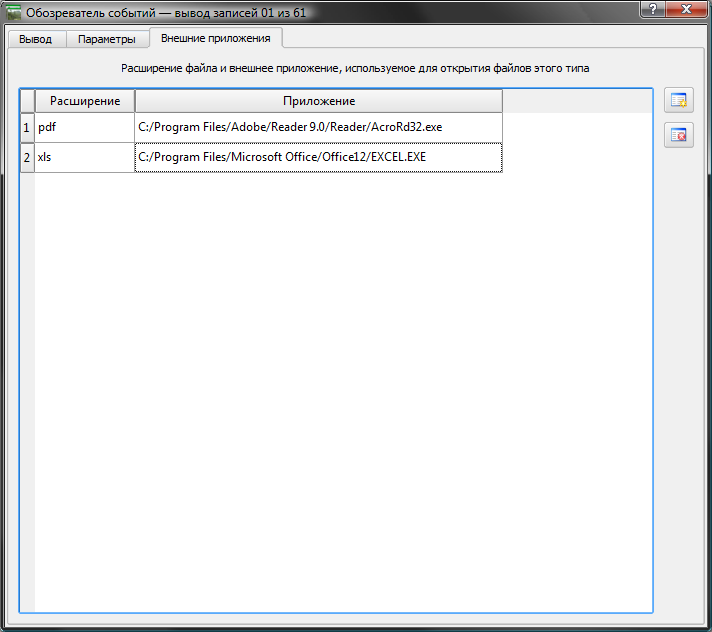
\includegraphics[clip=true, width=12cm]{evisexternal}
   \caption{La scheda applicazioni esterne di \emph{eVis} \nixcaption}\label{evisexternal}
\end{figure}

\begin{itemize}[label=--]
\item \textbf{(A) Tabella riferimento file}: una tabella contenente i vari tipi di file utilizzati da eVis.
Ogni tipo file necessita di un'estensione e di un percorso all'applicazione in grado di
gestirlo. Ciò permette di aprire diversi tipi di file come filmati, suoni e documenti testuali, oltre che 
solo immagini.
\item \textbf{(B) Aggiungi nuovo tipo file}: aggiunge un nuovo tipo di file (estensione ed applicazione).
\item \textbf{(C) Elimina riga corrente}:  elimina il tipo di file selezionato in tabella.
\end{itemize}

\minisec{Specificare la localizzazione ed il nome di una foto}\label{evis_specifying}

La localizzazione ed il nome di una foto possono essere memorizzati tramite un percorso relativo o assoluto
o tramite un URL se la foto risiede su un server web: seguono degli esempi dei vari approcci (Tabella \ref{tab:evis_examples}).

\begin{table}[htp]\index{plugins!evis}
\centering
\caption{Esempio con percorso assoluto, percorso relativo ed URL}\label{tab:evis_examples}\medskip
 \begin{tabular}{|p{0.55in}|p{0.55in}|p{4.7in}|p{0.7in}|}
 \hline \textbf{X} & \textbf{Y} & \textbf{FILE} & \textbf{BEARING}\\
 \hline 780596 & 1784017 & \filename{C:\textbackslash Workshop\textbackslash
eVis\_Data\textbackslash groundphotos\textbackslash DSC\_0168.JPG} & 275\\
 \hline 780596 & 1784017 & \filename{/groundphotos/DSC\_0169.JPG} & 80\\
 \hline 780819 & 1784015 &
\filename{http://biodiversityinformatics.amnh.org/evis\_test\_data/DSC\_0170.JPG} & 10\\
 \hline 780596 & 1784017 & \filename{pdf:http://www.testsite.com/attachments.php?attachment\_id-12}
& 76\\
 \hline
\end{tabular}
\end{table}

\minisec{Specificare la localizzazione ed il nome di altri documenti}\label{evis_location}

Altri documenti come testo, video e audio possono essere visualizzati e gestiti da eVis, basta
assicurarsi di aver impostato per ogni tipo di file estensione e applicazione nella scheda 
\tab{Configura applicazioni esterne} della finestra di dialogo \dialog{Browser evento}; è, inoltre,
necessario disporre del percorso o URL del file nella tabella attributi di un layer vettoriale.
Come regola addizionale, se l'URL non contiene l'estensione del tipo file, è possibile anteporre
l'estensione all'URL secondo il formato \texttt{estensione:URL}.
L'URL è preceduto dall'estensione file e dal segno : (due punti) (Tabella \ref{tab:evis_examples}).

\minisec{Utilizzo del Browser evento}\label{evis_using_browser}
 
Se tutto è correttamente impostato, lanciando il \dialog{Browser evento} verrà visualizzata un foto.
Se nella tabella attributi si fa riferimento ad un documento (o ad un'immagine in un formato non
supportato da eVis) ed il tipo di file è stato configurato nella scheda \tab{Configura applicazioni esterne}, 
il campo contente il percorso al file è evidenziato in verde: per aprire il documento, fare doppio-click 
sul testo evidenziato in verde.

Un asterisco rosso compare sull'elemento vettoriale associato ad una foto se non si è specificato 
l'orientamento della fotocamera. Nel caso contrario, viene visualizzata una freccia indicante la direzione. 

\subsection{Strumento ID evento}\label{evis_id_tool}

Il modulo 'ID evento' permette di visualizzare una foto cliccando su un elemento nella vista mappa di QGIS.
L'elemento vettoriale deve avere associati gli attributi contenenti la localizzazione ed il nome del file
della foto: il layer deve essere caricato in QGIS prima di aprire il modulo.

\minisec{Aprire ID Evento}\label{evis_launch_id}

Per aprire il modulo cliccare su \toolbtntwo{event_id}{Strumento ID evento} oppure \mainmenuopt{Plugins} \arrow 
\dropmenuopt{eVis} \arrow \dropmenuopt{Strumento ID evento}: sul cursore del mouse apparirà una ``i'', ad indicare che
lo strumento è attivo.

Per visualizzare le foto associate agli elementi vettoriali presenti nella vista mappa di QGIS, cliccare su
un elemento di interesse; la foto verrà mostrata nel 'Browser evento'. Nel caso fossero disponibili più foto
per lo stesso punto, è comunque possibile scorrerle tutte tramite i pulsanti Precedente e Avanti. 

\subsection{Connessione database eVis}\label{evis_database}

Il modulo Connessione Database permette di connettersi ed interrogare un database o altre risorse ODBC, es. un foglio di calcolo.

eVis può connettersi direttamente a quattro tipi di database: Microsoft Access, PostgreSQL, MySQL, SQLITE.
Può leggere dati da connessioni ODBC (es. una tabella Excel): in tal caso è necessario configurare il driver ODBC 
per il sistema operativo in uso.

\minisec{Aprire Connessione Database}\label{evis_launch_database}

Per aprire il modulo cliccare su \toolbtntwo{evis_connect}{Connessione database eVis} oppure \mainmenuopt{Plugins} \arrow 
\dropmenuopt{eVis} \arrow \dropmenuopt{Connessione database eVis}. 

La finestra di dialogo \dialog{Connessione Database} presenta tre schede: \tab{Query Predefinite}, \tab{Connessione Database},
\tab{Query SQL}. 
La 'Console di output' mostra lo stato di un'azione avviata da altre sezioni del modulo.

\minisec{Connessione Database}\label{evis_connect_database}

Aprire la scheda \tab{Connessione Database},  cliccare su \dropmenuopt{Tipo Database} ed inserire 
nome utente e password se richiesto. Inserire il server del database in 'Host Database': l'opzione 
non è disponibile per i database ``MSAccess''. Se il database si trova sul desktop, allora inserire 
``localhost''. Inserire il nome del database. In caso di connessione ``ODBC'' è necessario inserire il
nome della fonte dati.

Una volta configurati tutti i parametri cliccare su \button{Connetti}: la Console di Output informa 
dell'esito dell'operazione, sia positivo che negativo. 

\begin{figure}[ht]
   \centering
   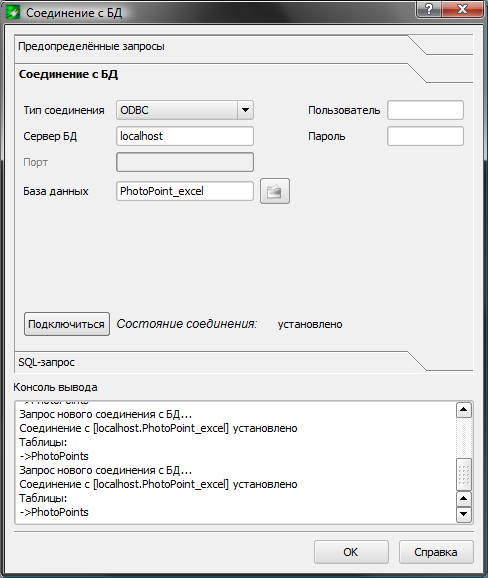
\includegraphics[clip=true, width=12cm]{evisdatabase}
   \caption{La scheda Connessione Database di \emph{eVis} \wincaption}\label{evisdatabase}
\end{figure}

\begin{itemize}[label=--]
\item \textbf{(A) Tipo di Database}: per specificare il tipo di database cui connettersi.
\item \textbf{(B) Host Database}: nome host del database.
\item \textbf{(C) Porta}: numero della porta di connessione in caso di database MYSQL o PostgreSQL.
\item \textbf{(D) Nome Database}: nome del database.
\item \textbf{(E) Connetti}:  pulsante di connessione.
\item \textbf{(F) Console di Output}: finestra dei messaggi sullo stato della connessione.
\item \textbf{(G) Nome utente}: nome utente in caso di database protetto.
\item \textbf{(H) Password}: password in caso di database protetto.
\item \textbf{(I) Query Predefinite}: scheda ``Query Predefinite''.
\item \textbf{(J) Connessione Database}: scheda ``Connessione Database''.
\item \textbf{(K) Query SQL}: scheda ``Query SQL''.
\item \textbf{(L) Help}: mostra la guida in linea.
\item \textbf{(M) OK}: chiude \dialog{Connessione Database}.
\end{itemize}

\minisec{Eseguire query SQL}\label{evis_running_sql}

Le query SQL permettono di estrarre informazioni da un database o da una risorsa ODBC. In eVis il 
risultato di una query è una layer vettoriale aggiunto alla vista mappa di QGIS.
Cliccare su \tab{Query SQL} per visualizzare l'interfaccia per le query. Un utile tutorial sulla 
sintassi SQL è disponibile alla pagina web \url{http://www.w3schools.com/sql/}. 
Ad esempio, per estrarre tutti i dati da una tabella Excel:

\begin{verbatim}
  select * from [sheet1\$]
\end{verbatim} 

dove ``sheet1'' è il nome del foglio di lavoro.

Per eseguire una query cliccare su \button{Esegui Query}: in caso di esito positivo si aprirà la finestra di
dialogo \dialog{Scegli file Database}, altrimenti la Console di Output mostrerà un messaggio di errore.

Nella finestra 'Scegli file Database' assegnare un nome al nuovo layer che sarà creato dai risultati della 
query.

\begin{figure}[ht]
   \centering
   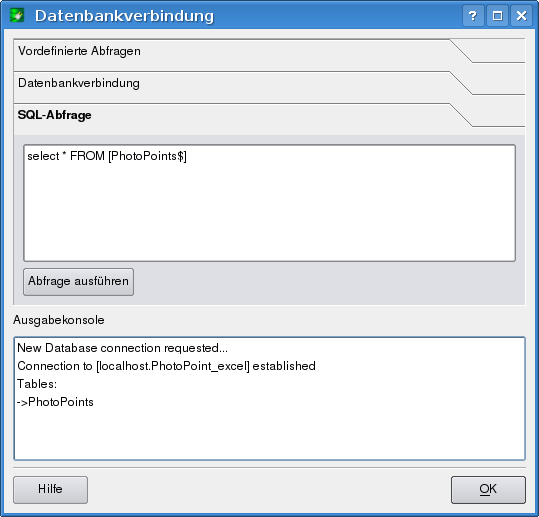
\includegraphics[clip=true, width=12cm]{evissql_query}
   \caption{La scheda Query SQL di \emph{eVis} \wincaption}\label{evissql_query}
\end{figure}

\begin{itemize}[label=--]
\item \textbf{(A) Query SQL}: è il riquadro per inserire le query SQL.
\item \textbf{(B) Esegui Query}: pulsante per mandare in esecuzione una query.
\item \textbf{(C) Console di Output}: mostra i messaggi relativi all'esecuzione delle query.
\item \textbf{(D) Help}: mostra la guida in linea.
\item \textbf{(E) OK}: chiude \dialog{Connessione Database}.
\end{itemize}

Usare \dropmenuopt{Coordinata X} e \dropmenuopt{Coordinata Y} per selezionare i campi del database 
che contengono le coordinate ``X'' (o longitudine) e ``Y'' (o latitudine). 
Cliccare su \button{OK} per visualizzare il nuovo layer nella vista mappa di QGIS.

Per salvare il nuovo layer è possibile usare il comando QGIS ``Salva con nome...'' (click tasto-destro
sul nome del layer in legenda).

\begin{Tip}\caption{\textsc{Creare un layer vettoriale da un foglio di lavoro Microsoft Excel}}
Quando si crea un layer vettoriale da un file Excel potrebbero notarsi degli (``0'') non voluti 
in alcune righe nella tabella degli attributi: la causa è da rilevarsi nell'abitudine di cancellare 
valori in Excel tramite il tasto ``backspace''. Per correggere il problema, bisogna aprire il Excel
e usare Modifica \arrow Elimina per rimuovere le righe non necessarie dal file.
\end{Tip}

\minisec{Eseguire query predefinite}\label{evis_predefined}

Nella scheda \tab{Query Predefinite} è possibile caricare query da file esterni in XML.
Cliccare su \tab{Query Predefinite} per aprire l'interfaccia delle query predefinite.

Per caricare query predefinite, cliccare su \toolbtntwo{evis_file}{Apri File}: quando una query è caricata,
il titolo della stessa appare nel menu a tendina sotto \toolbtntwo{evis_file}{Apri File} e una breve
descrizione è visualizzata nella casella di testo sottostante.

Selezionare la query che si intende usare e aprire la scheda \tab{Query SQL}: cliccare su \button{Esegui query} 
ed attendere i risultati. 

\begin{figure}[htp]
   \centering
   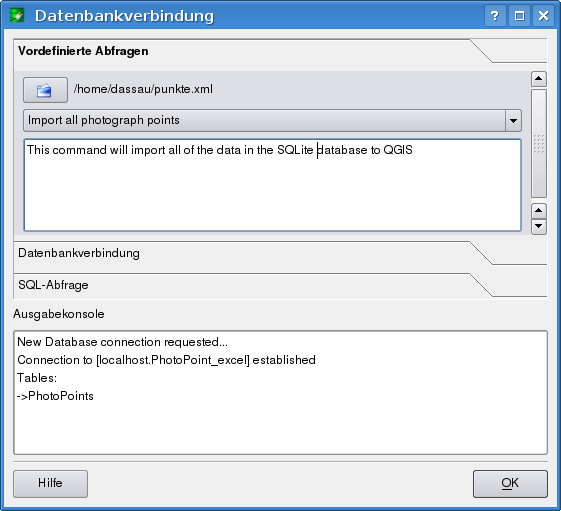
\includegraphics[clip=true, width=10cm]{evispredefined}
   \caption{Scheda Query Predefinite di \emph{eVis} \wincaption}\label{evispredefined}
\end{figure}

\begin{itemize}[label=--]
\item \textbf{(A) Apri File}: permette di selezionare il file XML contenente le query predefinite.
\item \textbf{(B) Query predefinite}: elenco delle query disponibili nel file XML.
\item \textbf{(C) Descrizione query}: breve descrizione della query derivata dal file XML.
\item \textbf{(D) Console di Output}: mostra messaggi relativi al processo in corso.
\item \textbf{(E) Help}: mostra la guida in linea.
\item \textbf{(F) OK}: chiude \dialog{Connessione Database}.
\end{itemize}

\minisec{Formato XML per le query predefinite di eVis}\label{evis_xml_format}

\begin{table}[htp]\index{plugins!evis}
\centering
\caption{Tag XML letti da eVis}\label{tab:evis_xml_tags}\medskip
 \begin{tabular}{|p{1.2in}|p{4.7in}|}
 \hline \textbf{Tag} & \textbf{Descrizione}\\
 \hline query & Definisce l'inizio e la fine di una istruzione di query.\\
 \hline shortdescription & Breve descrizione della query che viene mostrata nel menu a tendina di eVis.\\
 \hline description & Descrizione più dettagliata che viene mostrata nella casella 'Descrizione query' di eVis.\\
 \hline databasetype & Tipo di database come definito in 'Tipo Database' nella scheda \tab{Connessione Database}.\\
 \hline databaseport & La porta di connessione come definito in 'Porta' nella scheda \tab{Connessione Database}.\\
 \hline databasename & Il nome del database come definito in 'Nome Database' nella scheda \tab{Connessione Database}.\\
 \hline databaseusername & Nome utente come definito in 'Nome utente' nella scheda \tab{Connessione Database}.\\
 \hline databasepassword & Password come definito in 'Nome utente' nella scheda \tab{Connessione Database}.\\
 \hline sqlstatement & Il comando SQL.\\
 \hline autoconnect & Valore ``true''(vero) o ``false''(falso): in caso di ``true'', i tag sopra elencati saranno usati per connettersi automaticamente al database, senza avviare la procedura di \tab{Connessione Database}.\\
 \hline
\end{tabular}
\end{table}

Segue un esempio completo di file XML contenente tre query:

\begin{verbatim}
<?xml version="1.0"?>
<doc>
 <query>
   <shortdescription>Import all photograph points</shortdescription>
   <description>This command will import all of the data in the SQLite database to QGIS
      </description>
   <databasetype>SQLITE</databasetype>
   <databasehost />
   <databaseport />
   <databasename>C:\textbackslash Workshop/textbackslash
eVis\_Data\textbackslash PhotoPoints.db</databasename>
   <databaseusername />
   <databasepassword />
   <sqlstatement>SELECT Attributes.*, Points.x, Points.y FROM Attributes LEFT JOIN
      Points ON Points.rec_id=Attributes.point_ID</sqlstatement>
   <autoconnect>false</autoconnect>
 </query>
  <query>
   <shortdescription>Import photograph points "looking across Valley"</shortdescription>
   <description>This command will import only points that have photographs "looking across
      a valley" to QGIS</description>
   <databasetype>SQLITE</databasetype>
   <databasehost />
   <databaseport />
   <databasename>C:\Workshop\eVis_Data\PhotoPoints.db</databasename>
   <databaseusername />
   <databasepassword />
   <sqlstatement>SELECT Attributes.*, Points.x, Points.y FROM Attributes LEFT JOIN
      Points ON Points.rec_id=Attributes.point_ID where COMMENTS='Looking across
      valley'</sqlstatement>
   <autoconnect>false</autoconnect>
 </query>
 <query>
   <shortdescription>Import photograph points that mention "limestone"</shortdescription>
   <description>This command will import only points that have photographs that mention
      "limestone" to QGIS</description>
   <databasetype>SQLITE</databasetype>
   <databasehost />
   <databaseport />
   <databasename>C:\Workshop\eVis_Data\PhotoPoints.db</databasename>
   <databaseusername />
   <databasepassword />
   <sqlstatement>SELECT Attributes.*, Points.x, Points.y FROM Attributes LEFT JOIN
      Points ON Points.rec_id=Attributes.point_ID where COMMENTS like '%limestone%'
      </sqlstatement>
   <autoconnect>false</autoconnect>
 </query>
</doc>
\end{verbatim}

\FloatBarrier
